\documentclass[]{article}
\usepackage{lmodern}
\usepackage{amssymb,amsmath}
\usepackage{ifxetex,ifluatex}
\usepackage{fixltx2e} % provides \textsubscript
\ifnum 0\ifxetex 1\fi\ifluatex 1\fi=0 % if pdftex
  \usepackage[T1]{fontenc}
  \usepackage[utf8]{inputenc}
\else % if luatex or xelatex
  \ifxetex
    \usepackage{mathspec}
  \else
    \usepackage{fontspec}
  \fi
  \defaultfontfeatures{Ligatures=TeX,Scale=MatchLowercase}
\fi
% use upquote if available, for straight quotes in verbatim environments
\IfFileExists{upquote.sty}{\usepackage{upquote}}{}
% use microtype if available
\IfFileExists{microtype.sty}{%
\usepackage{microtype}
\UseMicrotypeSet[protrusion]{basicmath} % disable protrusion for tt fonts
}{}
\usepackage[margin=1in]{geometry}
\usepackage{hyperref}
\hypersetup{unicode=true,
            pdftitle={Reducing Measurement Error in List Experiments},
            pdfauthor={Mattias Agerberg and Marcus Tannenberg},
            pdfborder={0 0 0},
            breaklinks=true}
\urlstyle{same}  % don't use monospace font for urls
\usepackage{graphicx,grffile}
\makeatletter
\def\maxwidth{\ifdim\Gin@nat@width>\linewidth\linewidth\else\Gin@nat@width\fi}
\def\maxheight{\ifdim\Gin@nat@height>\textheight\textheight\else\Gin@nat@height\fi}
\makeatother
% Scale images if necessary, so that they will not overflow the page
% margins by default, and it is still possible to overwrite the defaults
% using explicit options in \includegraphics[width, height, ...]{}
\setkeys{Gin}{width=\maxwidth,height=\maxheight,keepaspectratio}
\setlength{\emergencystretch}{3em}  % prevent overfull lines
\providecommand{\tightlist}{%
  \setlength{\itemsep}{0pt}\setlength{\parskip}{0pt}}
\setcounter{secnumdepth}{0}
% Redefines (sub)paragraphs to behave more like sections
\ifx\paragraph\undefined\else
\let\oldparagraph\paragraph
\renewcommand{\paragraph}[1]{\oldparagraph{#1}\mbox{}}
\fi
\ifx\subparagraph\undefined\else
\let\oldsubparagraph\subparagraph
\renewcommand{\subparagraph}[1]{\oldsubparagraph{#1}\mbox{}}
\fi

%%% Use protect on footnotes to avoid problems with footnotes in titles
\let\rmarkdownfootnote\footnote%
\def\footnote{\protect\rmarkdownfootnote}

%%% Change title format to be more compact
\usepackage{titling}

% Create subtitle command for use in maketitle
\providecommand{\subtitle}[1]{
  \posttitle{
    \begin{center}\large#1\end{center}
    }
}

\setlength{\droptitle}{-2em}

  \title{Reducing Measurement Error in List Experiments}
    \pretitle{\vspace{\droptitle}\centering\huge}
  \posttitle{\par}
  \subtitle{Pre-analysis plan}
  \author{Mattias Agerberg and Marcus Tannenberg}
    \preauthor{\centering\large\emph}
  \postauthor{\par}
      \predate{\centering\large\emph}
  \postdate{\par}
    \date{03 November 2019}

\usepackage{booktabs}
\usepackage{longtable}
\usepackage{array}
\usepackage{multirow}
\usepackage{wrapfig}
\usepackage{float}
\usepackage{colortbl}
\usepackage{pdflscape}
\usepackage{tabu}
\usepackage{threeparttable}
\usepackage{threeparttablex}
\usepackage[normalem]{ulem}
\usepackage{makecell}
\usepackage{xcolor}

\usepackage{setspace}
\usepackage{bbm}
\doublespacing
\usepackage[utf8]{inputenc}
\usepackage{CJKutf8}

\begin{document}
\maketitle

\hypertarget{abstract}{%
\section{Abstract}\label{abstract}}

The \emph{list experiment} is one of the most important tools in social
science for eliciting truthful responses to sensitive questions. Under
some basic assumptions the list experiment can provide an unbiased
estimate of the share of affirmative answers to a sensitive question in
the population of interest. A drawback of the standard design is that
this estimate tends to have high variance. Recent studies also suggest
that non-strategic respondent error stemming from inattentive
respondents can be especially problematic in list experiments.
Inattentive respondents can both further increase variance and
substantially increase bias in the estimate of interest. This project
aims at developing and testing design-based solutions and
recommendations to minimize respondent error in list experiments. We
explore four different techniques to increase the average respondent
attention in the sample: Instructional manipulation checks; Factual
manipulation checks; the inclusion of a Placebo Statement in the control
list; and the inclusion of an Audit Warning to increase respondent
attentiveness. We discuss the upsides and challenges with respect to
each strategy as applied to the list experiment specifically. To
empirically evaluate the different methods we design several list
experiments where the true population quantity of the item of interest
(the ``sensitive'' item) is known. We use these to test the accuracy of
the list experiment in estimating the known quantity, and to explore the
potential of different methods to improve the quality of provided
responses. We end by discussing recommendations for applied researchers.

\newpage

\hypertarget{introduction}{%
\section{Introduction}\label{introduction}}

In recent years, the \emph{list experiment} has become one of the most
important tools in social science to elicit truthful responses to
sensitive questions. Under some basic assumptions, the list experiment
can provide an unbiased estimate of the share of affirmative answers to
a sensitive question in the population of interest. A drawback of the
standard design is that this estimate tends to be quite variable - a
consequence of the fact that the estimate is obtained by aggregating the
sensitive item with a list of non-sensitive items, where the sensitive
item is only given to half of the respondents (the treatment group).
This has spurred a large body of work on efficient statistical
estimation of the quantity of interest (Aronow et al. 2015; Blair and
Imai 2012; Corstange 2009; Imai 2011; Tian et al. 2017).

However, all estimation techniques are typically sensitive to different
types of respondent error (Ahlquist 2018; Blair, Chou, and Imai 2019).
\emph{Strategic} respondent error in list experiments, where the
respondent for instance might avoid selecting the maximum or minimum
number of items, can generally be minimized by choosing control items
(non-sensitive items) in a well-thought-out manner (Glynn 2013).
\emph{Non-strategic} respondent error, on the other hand, arises when
respondents provide a \emph{random} response to the list experiment.
Given that the list lengths differ between the treatment and control
group, this type of error will often be correlated with the treatment
and can hence dramatically increase both bias and variance in the
estimate of interest (Ahlquist 2018).

Non-strategic respondent error is likely to be high when respondents do
not pay enough attention to the survey (Berinsky, Margolis, and Sances
2014). As many survey experiments nowadays are conducted using online
platforms like MTurk, making sure respondents actually provide
meaningful responses has become increasingly difficult. While the issue
of low respondent effort and attention is well-known, researchers often
do not consider it when analyzing their experiments (Harden, Sokhey, and
Runge 2018). Given the challenges to efficient analysis of list
experiments in the first place (see Blair, Coppock, and Moor (2018) for
an overview), we should expect these issues to be especially pronounced
here. Recent research suggests that this might indeed be the case
(Alvarez et al. 2019).

This project aims at developing and testing design-based solutions and
recommendations to minimize respondent error in list experiments. In
particular, we explore a number of techniques from previous research to
raise the average attentiveness in the sample, including instructive
manipulation checks (Berinsky, Margolis, and Sances 2014; Oppenheimer,
Meyvis, and Davidenko 2009), and a ``warning message'' to increase
respondent attentiveness (Clifford and Jerit 2015). We also extend
existing methods by developing a factual manipulation check for the list
experiment and techniques to include a placebo item in the control list.

To be able to evaluate the different methods and criteria for excluding
inattentive respondents, we design several list experiments where the
item of interest (the ``sensitive'' item) has three specific properties:
(1) the true quantity of the item is known, (2) the item is independent
of all items on the control list, (3) the item is independent of all
(observed and unobserved) respondent characteristics. We construct
``sensitive'' items that meet these criteria by randomly selecting an
item from a list of items for each individual respondent. This way, the
expected prevalence for the ``sensitive'' item on the list is known by
design. We then compare different methods and criteria by estimating the
root mean squared error of the prediction for the item of interest (a
quantity we define below).

This project contributes to the literature on survey methodology in
general and to the growing literature on list experiments in particular.

\hypertarget{methods-to-reduce-non-strategic-respondent-error-in-list-experiments}{%
\section{Methods to reduce non-strategic respondent error in list
experiments}\label{methods-to-reduce-non-strategic-respondent-error-in-list-experiments}}

In this section we briefly describe the different methods to reduce
respondent error that we consider in the study at hand. First, we
consider standard ``manipulation checks'' (or ``screeners''). A common
type of manipulation check is the instructional manipulation check (IMC)
(Oppenheimer, Meyvis, and Davidenko 2009). IMCs work by instructing
respondents to show that they are paying attention. This is done by
giving respondents a precise set of instructions to follow when
responding to the IMC items which are embedded in the survey.
Respondents failing to follow the instructions are classified as
``inattentive'' and potentially excluded from the data analysis
(Berinsky, Margolis, and Sances 2014). We also consider a second type of
manipulation check that instead asks objective questions about key
elements in the experiment. This type of manipulation check, referred to
as a factual manipulation check (FMC), thus aims to identify individual
attentiveness to experimental information directly (Kane and Barabas
2019). Below we design an FMC that is specifically tailored to the list
experiment.

Another option to potentially improve the estimate of interest is to
include a \emph{placebo} item in the control list that equalizes the
lists' length. If respondents answer in a manner that is correlated with
the list length, for instance by using the total number of items on the
list as a ``reference point'' (De Jonge and Nickerson 2014), this will
bias standard estimators for the prevalence of the sensitive item.
Equalizing the lists thus removes the bias created by some forms of
non-strategic respondent error, something that we discuss further below.
A placebo item in this sense is an item where the true population
quantity is zero. The item should hence only increase the length of the
control list, without changing the expected number of affirmative
responses to the control items in the population (Riambau and Ostwald
2019). This strategy theoretically eliminates some types of bias
emanating from the different list lengths. However, good placebo items
can be difficult to design and implement. We discuss this problem and
propose novel solutions below.

Both the IMC and the FMC can be used to identify shirking respondents.
It is not, however, always obvious what to do with these. Excluding a
large number of respondents might be problematic - especially if done in
a careless manner (Aronow, Baron, and Pinson 2019; Berinsky, Margolis,
and Sances 2014). A final strategy we consider is therefore to try to
\emph{increase} the average respondent attentiveness. A simple
intervention explored by Clifford and Jerit (2015) is to provide a
``warning message'' to the respondents. This is a short message stating
that responses are carefully checked and that only responses from
participants that demonstrate that they have read and understood the
survey will be used. The respondents also have to indicate that they
have understood the instructions. The authors find that respondents
given this message (referred to as ``audit'' in the study) are
substantially more attentive than respondents in the control group who
received no message.\footnote{The authors try several different warning
  messages but find the ``audit'' message to be the most effective.}

\hypertarget{setup-and-some-simulation-evidence}{%
\section{Setup and some simulation
evidence}\label{setup-and-some-simulation-evidence}}

Before turning to the empirical study, we provide some simulation
evidence to demonstrate the potential effectiveness of the methods
discussed above. The list experiment works by aggregating a sensitive
item with a list of control items to protect respondents' integrity
(Glynn 2013). We adopt the notation in Blair and Imai (2012) and
consider a list experiment with \(J\) binary control items and one
binary sensitive item denoted \(Z_{i, J+1}\). Respondents are randomly
assigned to either a control group (\(T_{i}=0\)) and given the list with
\(J\) control items, or to a treatment group (\(T_{i}=1\)), given the
list with with \(J\) control items \emph{and} the sensitive item
\(Z_{i, J+1}\). The total number of items in the treatment group is thus
\(J+1\). \(Y_{i}\) denotes the observed response to the list experiment
for respondent \(i\) (the total number of items answered affirmatively).
If we denote the total number of affirmative answers to \(J\) control
items with \(Y^*_{i}\), the process generating the observed response can
be written as: \[
Y_{i} = T_{i}Z_{i, J+1} + Y^*_{i}
\] Blair and Imai (2012) show that if we assume that the responses to
the sensitive item are truthful (``no liars'') and that the addition of
the sensitive item does not alter responses to the control items (``no
design effects''), the proportion of affirmative answers to the
sensitive item, denoted \(\tau\), can be estimated by taking the
difference between the average response among the treatment group and
the average response among the control group (i.e.~a difference-in-means
estimator (DiM)).\footnote{The difference-in-means estimator can be
  written as: \[
    \hat{\tau} = \frac{1}{N_{1}} \sum_{i=1}^{N}T_{i}Y_{i} - \frac{1}{N_{0}} \sum_{i=1}^{N}(1-T_{i})Y_{i}
    \] \noindent where \(\hat{\tau}\) is the estimated proportion
  affirmative answers to the sensitive item,
  \(N_{1} = \sum_{i=1}^{N}T_{i}\) is the size of the treatment group and
  \(N_{0}=N-N_{1}\) is the size of the control group.}

Inattentive respondents potentially violate both assumptions if they
provide a \emph{random} response to the list experiment. For
illustration, we simulate one basic method to decrease non-strategic
respondent error: excluding respondents who fail manipulation checks.
The basic simulation assumes 2000 respondents. The control list consists
of 4 independent items, each drawn from a Bernoulli distribution. The
parameter \(p_{j}\) was set to 0.5, 0.5, 0.15, and 0.85 for the
different items respectively. In line with current recommendations
(Glynn 2013), two of the control items were generated to be negatively
correlated (\(r=-0.6\)). The treatment list consists of the same 4 items
plus a ``sensitive'' treatment item, drawn from a Bernoulli distribution
with \(p=\frac{1}{6}\). This basic setup is very close to the setup used
in Ahlquist (2018) and Blair, Chou, and Imai (2019). In the appendix we
discuss and show how changes to the setup affect the simulation results.

25\% of the total number of ``respondents'' were randomly assigned to be
``inattentive'' (for instance, Alvarez et al. (2019) estimates that 36\%
of respondents in their experiment were inattentive, and from an earlier
application of the list experiments in a similar setting we estimate
28\% of respondents to be inattentive (Robinson and Tannenberg 2019)).
Throughout the paper we denote the share of inattentive respondents with
\(s\). We simulate a process where inattentive respondents answer
randomly: for inattentive respondents in the control group the outcome
was replaced by a draw from a discrete uniform distribution,
\(U\{0,4\}\), and the outcome for the inattentive treatment group was
replaced by a draw from \(U\{0,5\}\). Blair, Chou, and Imai (2019) argue
that this is a plausible model for the behavior of inattentive
respondents answering the list experiment. We refer to this as the
\emph{uniform error model}. If we set \(W_{i}\) equal to 1 to indicate
that a specific respondent is inattentive (0 otherwise), the process
generating the observed response under this model can be written as: \[
Y_{i} = (1-W_{i})(T_{i}Z_{i, J+1}+Y^*_{i})+W_{i}(T_{i}U_{\{0,J+1\}}+(1-T_{i})U_{\{0,J\}})
\] The conseqeunces of this error process in terms of bias in the
estimate of \(\tau\) are similar to several other plausible error
processes. We discuss this further in the appendix.

To simulate a successful manipulation check we then randomly exclude a
share of the ``inattentive'' respondents. This share is denoted by
\(s'\). Figure \ref{sim_excluded} shows the distribution of
\(\hat{\tau}\) based on 10000 simulated data sets (assuming the setup
described above) for different \(s'\): no inattentives excluded
(\(s'=0\); purple), an ineffective attention check (\(s'=0.3\); teal),
and an effective attention check (\(s'=0.8\); yellow). As shown in
figure \ref{sim_excluded}, the mean \(\hat{\tau}\) is just above 0.266
when no inattentive respondents are excluded (purple). Considering that
we are trying to estimate an item with a prevalence of \(\frac{1}{6}\),
this is a full 10 percentage points off from the true
prevalence.\footnote{As shown by Blair, Chou, and Imai (2019), under the
  uniform error model the bias in the DiM estimator will be
  \(s \left(\frac{1}{2} - \tau \right)\), which amounts to 0.1 in the
  simulation example.} Excluding inattentive respondents can clearly be
very beneficial under this setup. For instance, excluding 80\% of the
inattentive respondents (yellow) lowers the mean \(\hat{\tau}\) to
0.193, less than three percentage point off from the true prevalence.
Overall, this basic simulation shows that inattentive respondents in
list experiments can be hugely problematic, but also that the estimates
can be greatly improved by decreasing the share of inattentives in the
sample.

\begin{figure}
\centering
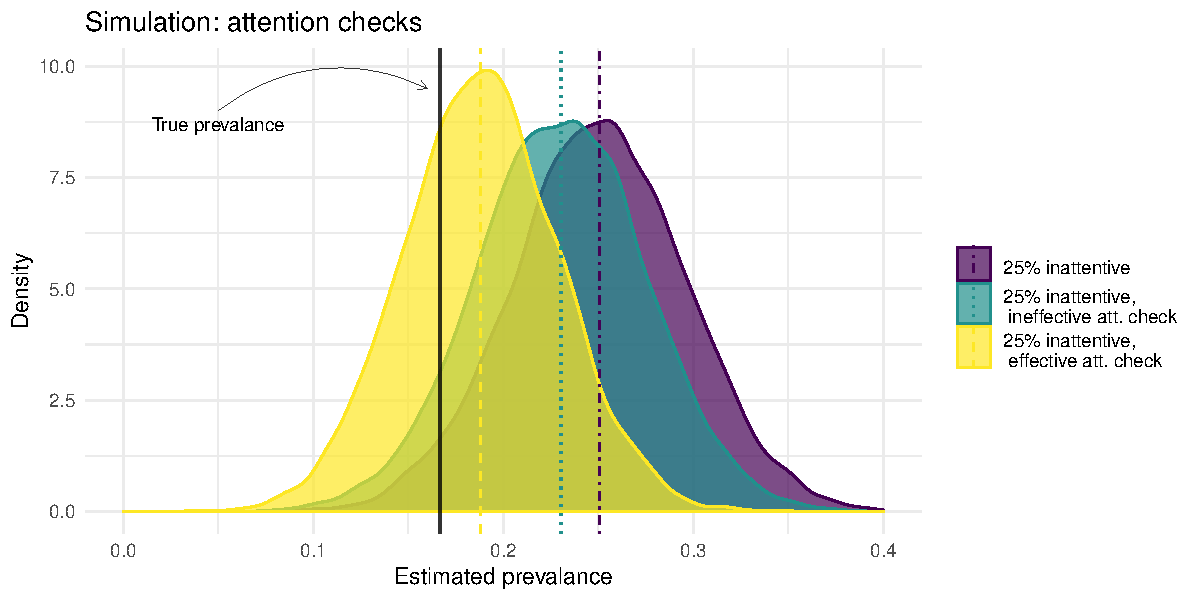
\includegraphics[width=6.25in,height=\textheight]{output/estimates_attention_checks_color.pdf}
\caption{Simulation of \(\hat{\tau}\) by exclusion of inattentive
respondents. 10000 simulated data sets. \label{sim_excluded}}
\end{figure}

\hypertarget{research-design}{%
\section{Research design}\label{research-design}}

This study evaluates several strategies to increase average respondent
attentiveness in data from list experiments as well as ways of reducing
the negative effects of respondent inattentiveness. The basic research
design consists of a set of two list experiments for which the item of
interest (the ``sensitive'' item) has three specific properties: (1) the
true quantity of the item is known, (2) the item is uncorrelated with
all items on the control list, (3) the item is uncorrelated to all
(observed and unobserved) respondent characteristics. This way, we can
calculate the bias and variance of different estimates for the item.
Moreover, we know that the expected prevalence of the item does not
change with the exclusion of some respondents or with the addition of a
specific control item. We compare the effectiveness of different
strategies to minimize respondent error by estimating the root mean
squared error of the prediction (pRMSE) for the ``sensitive'' item:

\[
pRMSE(\hat{\tau}) = \sqrt{Var(\hat{\tau}) + (\tau - \hat{\tau})^2}
\]

\noindent where \(\tau\) is the true quantity of interest (the true
prevalence of the item in the population) and \(\hat{\tau}\) is the
estimated quantity from the list experiment. This statistic hence
captures the trade-off between bias and variance in the list experiment.
Some strategies might reduce bias but at the same time increase the
variance of the estimate. Excluding inattentive respondents could, for
instance, have this effect.

Both list experiments consist of a set of four control items, where the
order in which they appear on the list is randomized (see full survey in
appendix for details). Following best practice, two of the items on each
list are negatively correlated (Glynn 2013).\footnote{The combination of
  control items on both lists have previously been used in a similar
  context and does appear to work well to avoid ceiling and floor
  effects (see Robinson and Tannenberg (2019)).} The order in which the
two lists appear are also randomized to guard against potential
``learning effects'' which otherwise risk limit the inferences we can
draw from comparing the various conditions.

For the first list experiment (A), the control list is randomly given to
half of the respondents. The other half receives the treatment list,
which consist of one additional, ``sensitive'' item. This item should
have the three features described above. In the first list we use a
statement about respondents' birth-timing within the year to construct a
``sensitive'' item with the three desired properties. The respondents
who are assigned the treatment list will receive a statement of being
born in one of the four seasons, for example, \emph{I was born in Winter
(Dec/Jan/Feb)}. The statement is randomly drawn from the four seasons
and piped into the list. Agreement with the proposed statement
(\(\tau\)) will therefore be one quarter (25 percent) in expectation.
This follows from the fact that exactly one out of the four potential
statements will be true for each respondent. The true population
quantity of the item will thus be known (1). Since whether or not the
item is true for a given respondent is random by construction, the
proposed item will also have property (2) and (3).

In the second list experiment (B), one third of the sample is randomly
assigned the basic four item control list. Another third receives the
control list \emph{plus} a placebo item, for which the true prevalence
by design is 0 (this is described in detail below). The remaining third
receives the control list plus a treatment item. In list B we employ
regarding ones zodiac animal, for example \emph{I was born in the year
of the Dog or in the year of the Pig.}, as the ``sensitive'' item. The
study will be fielded in China, where respondents' knowledge of their
zodiac animal is safe to assume. Each given year is associated with one
animal of which there are 12 in total. The specific animal combination
presented on the list to each respondent is randomly drawn from a list
of 6 different combinations and is piped into the question item (see
full survey in the appendix for the 6 zodiac statements). Hence,
agreement with the proposed item (\(\tau\)) is two twelfths (16.66
percent) in expectation for each respondent. Again, the population
quantity is therefore known (1), and given that the specific animal
combination is presented at random, the item will be uncorrelated to all
the control items on the list (2), as well as any respondent
characteristics.

The study will also include three additional list experiments, C, D, and
E applied to three sensitive items: C) ``I have trust in the national
government in Beijing''; D) ``I have trust in the local government'';
and E) ``I have witnessed an act of corruption or bribe-taking by a
government official in the past year''. List C, D and E will have same
set up as list B, with one third of the sample receiving the control
list, one third the control list plus a placebo, and one third the
treatment list. Although these lists cannot be used to directly test the
suggested solutions to minimize respondent error by comparing
\(pRMSE(\hat{\tau})\) (because the sensitive items do not fulfill the
properties (1), (2) or (3)), the lists still allow us to test the face
validity of some of the proposed approaches. For example, for the
sensitive item of having \emph{witnessed corruption} for which we expect
prevalence level to be fairly low,\footnote{In the latest round of the
  Asian Barometer only 6.7 percent of respondents report that that have
  witnessed corruption in the last year {[}CITE{]}. While we believe
  this is a sensitive item that suffers from underreporting the true
  prevalence rate should be well below 50 percent.} the estimate
\(\hat{\tau}\) obtained when the quantity is estimated using control
group 1 (with the placebo item) should be \emph{lower} than the estimate
obtained when using control group 2 (no placebo item) due to mechanical
inflation in the latter. Similarly, we would also expect the
\(\hat{\tau}\) obtained using control group 2 (no placebo item) to
decrease if we exclude inattentive respondents based on the IMC and/or
the FMC as long as the prevalence of the sensitive item is below 0.5.
From assuming inattentive respondents to select their response at random
(according to a uniform distribution) we expect the
\(\hat{\tau}_{inattentives} \approx 0.5\), thus their inclusion likely
bias \(\hat{\tau}\) upwards.\footnote{This follows from the fact that
  the expected value of a (discrete) uniform distribution is
  \(\frac{a+b}{2}\), where the interval \([a,b]\) denotes the support of
  the distribution. For a list experiment with \(J\) control items and
  one sensitive item where respondents answer according to a uniform
  distribution we get
  \(\mathbf{E}[Y_{i}|T_{i}=1] = \frac{0 + (J+1)}{2}\) for the treatment
  group, and \(\mathbf{E}[Y_{i}|T_{i}=0] = \frac{0 + J}{2}\) for the
  control group. The expected difference between the groups is thus
  \(\mathbf{E}[\tau_{inattentives}] = \mathbf{E}[Y_{i}|T_{i}=1] - \mathbf{E}[Y_{i}|T_{i}=0] = \frac{1}{2}\).}

\hypertarget{dealing-with-inattentive-respondents}{%
\subsection{Dealing with inattentive
respondents}\label{dealing-with-inattentive-respondents}}

We evaluate four different strategies to improve the average respondent
attentiveness in the sample: the IMC, the FMC, the inclusion of a
placebo item, and a warning message. The specific questions and
manipulations we use are described below.

\hypertarget{instructional-manipulation-check-imc}{%
\subsubsection{Instructional Manipulation Check
(IMC)}\label{instructional-manipulation-check-imc}}

First we will use standard Instructional Manipulation Checks (IMC) to
identify inattentive respondents. All respondents will receive two IMCs
adopted from Berinsky, Margolis, and Sances (2014) and Berinsky,
Margolis, and Sances (2019), one ``multiple choice screener'' and one
``grid screener''. These are minimally modified to suit our survey mode
(see appendix for full question wording). The first IMC requires
respondents to demonstrate that they are paying attention by following a
precise set of instructions about which alternative or action to select
at the end of a somewhat lengthy question (placed among the background
questions) (Berinsky, Margolis, and Sances 2014; Oppenheimer, Meyvis,
and Davidenko 2009). In second IMC (the grid screener) the respondent is
asked ``In the grid below you will see a series of statements. please
tell us whether you agree or disagree with each statement.'' The grid
contain seven statements in total out of which five are sincere
attitudinal statements. The remaining two probe for attentiveness and
read: ``Please click the''neither agree nor disagree" response" and
``Two is greater than one'', which both have a single correct answer.
The order of the seven statements is randomized.

We treat respondents who fail either one of the IMCs as inattentive.
Note that for passing the second IMC respondents have to pass both
screener statements in the grid. Excluding inattentives who fail IMCs
placed \emph{before} the list experiment will not introduce
post-treatment bias. It may however affect the representativeness of the
overall sample, which we will explore in the paper.

\hypertarget{factual-manipulation-check-fmc}{%
\subsubsection{Factual Manipulation Check
(FMC)}\label{factual-manipulation-check-fmc}}

We also consider a second type of manipulation check that instead asks
objective questions about key elements in the experiment. This type of
manipulation check, referred to as a factual manipulation check (FMC),
thus aims to identify individual attentiveness to experimental
information directly (Kane and Barabas 2019). We develop a FMC
specifically tailored to the list experiment and are mindful to
construct one that is not correlated with the treatment itself
(receiving the list with the item of interest) so as to minimize the
risk for post-treatment bias of analyses that conditions on the FMC (see
Aronow, Baron, and Pinson (2019)). The FMC reads:

\begin{quote}
You have just answered a question by selecting a number of items from a
list that you agree with. Below are four items. Only one of these were
featured on the previous list. Which one was it? Please select this item
irregardless of if this was one of the items you agreed with or not.
\end{quote}

To pass the FMC respondents will have to pick out the correct item from
a list items that are different in character from most items on the
list. We will also include an ``I don't remember'' response option to
minimize guessing among inattentive respondents. For example, for list A
the options are ``We should focus less on the economy and more on the
environment; I like pineapple very much; Our city needs another
amusement park; I live in an apartment building;'', presented in a
randomized order, and with the option ``I don't remember'' presented
last.

Our assumption is that this task is equally difficult regardless of
having seen a list with 4 (the control list) or 5 items (the treatment
list). Since the FMC is administered \emph{after} the list experiment,
dropping respondents based on passage of the FMC runs the risk of
introducing post-treatment bias if the character of the list (treatment
or control) would affect the result of the FMC (Aronow, Baron, and
Pinson 2019). While there is no perfect way to guard against the
possibility of post-treatment bias in this case, we propose two tests to
check if the assumption of \emph{no} post-treatment bias is plausible.
First, we regress a binary variable \(y\) that equals 1 for respondents
passing the FMC (0 otherwise) on an indicator variable \(T\) that equals
1 for respondents assigned to the treatment list and 0 otherwise. We use
logistic regression to estimate the equation and compute a LR-test to
see if the inclusion of \(T\) is an improvement over the null-model. A
rejection of the null-hypothesis in the LR-test would be evidence that
the passage rates on the FMC are not equal for the treatment and control
group in the list experiment. Second, we estimate the following logistic
regression model \emph{after} excluding respondents based on failure on
the FMC: \(logit(T_{FMC = 1}) = \mathbf{X'}_{FMC = 1}\beta + \epsilon\),
where \(T_{FMC = 1}\) is the treatment assignment in the list
experiment, \(\mathbf{X}_{FMC = 1}\) is a vector of pre-treatment
covariates, and \(\epsilon\) is the error term. We again compute a
LR-test to test the null-hypothesis that the coefficients in the vector
\(\beta\) are jointly equal to 0. This hence amounts to a ``balance
test'': does the exclusion of respondents due to failing the FMC create
imbalances on observed covariates between the treatment and control
group in the list experiment? As noted by Aronow, Baron, and Pinson
(2019), tests like these can merely give us an indication by (ideally)
not providing positive evidence in favor of post-treatment bias.
However, our experimental design also gives us the possibility to simply
check what happens when we condition on the FMCs: does this decrease
bias in the estimate of \(\tau\)? Together, these tests and explorations
allow us to evaluate the effectiveness of the FMCs and whether these are
likely to introduce post-treatment bias.

\hypertarget{reducing-list-effect-bias---placebo-statement}{%
\subsection{Reducing list effect bias - placebo
statement}\label{reducing-list-effect-bias---placebo-statement}}

Another option to potentially reduce the bias of the estimate of
interest is to include a \emph{placebo} item in the control list that
equalizes the lists' length. Equalizing the lists' length is a way to
guard against potential \emph{list effect bias} stemming purely from the
fact that one list (the treatment list) is longer than the other. Even
(somewhat) attentive respondents may interact with the list differently
only depending on whether they are assigned to a list with 4 or 5 items.
In the face of list effect bias \(Y^*_{i}\) might both be the function
of the true answers to the individual control items \emph{and} a
function of the list's length \(L_{J}\). For instance, some respondents
may use the number of items on the list to figure out how many items on
the list that ``should'' apply to them, for example by anchoring at the
mean number of items of the list, and then adjust from this value. Or
some respondents might use the maximum response to determine if a
certain low response (say 1) is ``too low''. In both these cases a
respondent might adjust a true low response upwards. In this sense the
total number of items on the list could work as a ``reference point''
for respondents (see De Jonge and Nickerson (2014) for on overview of
the psychological literature on such effects). We refer to such an
effect, where the respondent's reported answer to the list deviates from
their true aggregated preference for the items on the list, as a
\emph{list effect}.

In general, such list effects are not a problem as long as the effect is
the same for the treatment and control group (\(L_{J}=L_{J+1}\)). Given
that many of the proposed effects are directly related to the number of
items on the list (for instance, anchoring using the mean number), it is
not unreasonable to assume that \(L_{J} \neq L_{J+1}\). This would
create list effect bias in the estimate of \(\tau\) equal to
\(\Delta L\), where \(\Delta L = L_{J+1} - L_{J}\).\footnote{This would
  hence be a violation of the ``no design effects'' assumption.} In the
examples above \(\Delta L\) would be positive, leading to an
artificially inflated estimate of \(\tau\). Introducing a placebo item
on the control list thus makes \(\Delta L = L_{J+1} - L_{J+1} = 0\),
assuming that \(L_{J+1}\) is independent of both the placebo item and
the sensitive item. To obtain an unbiased estimate of \(\tau\) with the
DiM estimator the expected prevalence of the placebo item for each
respondent has to be 0.

Important to note is that list efect bias is different from the bias
created by inattentive respondents. In general, a placebo item is not
necessarily an optimal way of reducing bias stemming from inattentive
respondents. In the appendix we show that under the uniform error model,
the inclusion of a placebo item changes the bias in the DiM estimator
from \(s \left(0.5 - \tau \right)\) (no placebo) to \(-s\tau\)
(placebo). Rather, a placebo item has the potential to equalize any list
effects between the treatment and control group among \emph{attentive}
respondents.

Previous studies considering techniques to equalize the list length
between the treatment and the control group have not sufficiently
discussed the different implications this might have for inattentive and
attentive respondents (De Jonge and Nickerson 2014; Holbrook and
Krosnick 2010; Riambau and Ostwald 2019; Tsuchiya, Hirai, and Ono 2007).
Consider two different control lists, \(C_{J}\) and \(C_{J+pl}\). \(C\)
includes \(J\) control items and \(C_{J+pl}\) includes the same set of
control items plus a placebo item (where the true prevalence for each
respondent is 0). For respondents answer according to the uniform error
model the expected difference between these lists is \(s/2\). This
follows from the fact that the expected value of \(\tau\) for
inattentive respondents under this error model is \(1/2\) (see above).
Any test of potential list effect bias should therefore first try to
exclude all truly inattentive respondents; otherwise we have no way of
distinguishing list effect bias from bias created by inattentive
respondents. Testing for list effect bias would thus involve estimating
\(\mathbf{E}[Y_{i}|C_{J+pl}] - \mathbf{E}[Y_{i}|C_{J}]\), using the
sample of attentive respondents. If the estimated quantity is different
from 0, this is evidence in favor of list effect bias. In the presence
of such bias the inclusion of a placebo item in the control list can be
expected to decrease bias in the estimate of \(\tau\).

To explore whether the inclusion of a placebo item is warrented we need
an item for which the true expected prevalence for each respondent is 0.
Ideally such an item should be \emph{plausible} for all respondents, yet
by design \emph{necessarily false} for any one given respondent. We
propose a design for a placebo item that can be implemented in any
programmed survey, such as web-administrated or tablet-administrated
surveys, where it is possible to pipe in an item utilizing information
gained earlier in the survey. This can be done in a number of different
ways. In our application we will give survey respondents who indicate
that they are below 30 years of age the statement ``I was born in the
70s'', and respondents who indicate that they are 30 or above get the
placebo statement ``I was born in the 2000s''. To the best of our
knowledge this approach to assigning a placebo item is a novel
innovation. Theoretically this approach has one clear benefit vis-a-vis
existing approaches. For example, in the Singaporean setting Riambau and
Ostwald (2019) use ``I have been invited to have dinner with PM Lee at
Sri Temasek {[}the Prime Minister of Singapore's residence{]} next
week.'', which they suggest is ``plausible but false'' for all
respondents. The authors caution against using ridiculous items (such as
having the ability to teleport oneself) so as not to risk compromise the
perceived seriousness of the survey. We take this one step further and
suggest that there is a benefit to having an placebo item that is
\emph{truly} plausible to signal seriousness. Using an item that is
necessary true or necessary false due to \emph{implausibility} risks
signaling to the respondent that their responses are not important or
valuable to the researchers, which risk result in lower attentiveness.

We will explore the inclusion of a placebo item by randomly assigning
the placebo item to one third of the sample of list B, control group 1
(\(C_{J+pl}\)). Another third of the sample, control group 2
(\(C_{J}\)), get the basic control list containing the four items. The
remaining third of the sample get the treatment list. We will use the
same setup, with two control groups, for list experiment E. List
experiment B is designed according to the same principles as list
experiment A, with a ``sensitive'' item that has properties (1), (2),
and (3), while list experiment E has a sensitive item for the treatment
list. We will use list B and E to test for list effect bias. We will
first use the IMC to exclude exclude inattentive respondents. We will
then use the DiM estimator to estimate
\(\mathbf{E}[Y_{i, IMC=1}|C_{J+pl}] - \mathbf{E}[Y_{i, IMC=1}|C_{J}] = \hat{\Delta L}\).
We consider an estimated quantity that is statistically different from 0
to be evidence in favor of list effect bias. We will repeat this
procedure but instead using the FMCs to exclude respondents.\footnote{In
  addition, the placebo lists can also be used as a sanity check for the
  IMC and the FMC: if these exclusion criteria are good at identifying
  inattentive respondents they should reduce the number of respondents
  who answer ``5'' on the placebo lists to near 0.} If
\(\hat{\Delta L}\) is estimated to be statistically different from 0 in
one or more of these tests this is an indication that researchers should
consider including a placebo item in the control list. If we find
evidence in favor of list effect bias we will also compare the
\(pRMSE(\hat{\tau})\) for list experiment A when we use the two
different control lists respectively. In the presence of such bias we
expect this quantity to be lower when we use the placebo list. See the
appendix for a discussion of statistical power of tests pertaining to
the placebo item.

\hypertarget{improving-attentiveness-of-respondents---audit-check}{%
\subsection{Improving attentiveness of respondents - audit
check}\label{improving-attentiveness-of-respondents---audit-check}}

Finally, we also test the possibility of \emph{improving} the
attentiveness of respondents in the sample. In order to do this half of
the sample is randomly assigned to receive a ``warning message'' just
before being presented with the first list experiment. The other half of
the sample receive no message.\footnote{For all other analyses we simply
  average over this manipulation.} The message is taken from Clifford
and Jerit (2015) who develop and test several types of warning messages
and find that the ``audit'' message is the most effective in increasing
respondent attentiveness. This is a short message stating that responses
are carefully checked and that only responses from participants that
demonstrate that they have read and understood the survey will be used.
The respondents also have to indicate that they have understood the
instructions. The full question wording reads:

\begin{quote}
We check responses carefully in order to make sure that people have read
the instructions for the task and responded carefully. We will only
accept participants who clearly demonstrate that they have read and
understood the survey. Again, there will be some very simple questions
in what follows that test whether you are reading the instructions. If
you get these wrong, we may not be able to use your data. Do you
understand? {[}Yes, I understand; No, I do not understand{]}
\end{quote}

We analyze the effectiveness of the warning message in several ways.
First, we will estimate the effectiveness of the message by measuring
what fraction of respondents in each group that passes the FCMs. Since
the FMCs are directly related to the lists, this will give an overall
indication of whether the message plausibly increases the attention
respondents pay to the list experiments. We will also compare the
\(pRMSE(\hat{\tau})\) in the two list experiments (A and B) between the
treatment group (that received the message) and the control group. Given
that we are splitting the sample in half when comparing the two groups
(since we analyze the list experiment separately for the two groups),
this comparison has less statistical power. We discuss this more in
depth in the appendix.

\hypertarget{expectations-and-main-analysis}{%
\section{Expectations and main
analysis}\label{expectations-and-main-analysis}}

All our proposed methods aim to minimize non-strategic respondent error
or the consequences of such error. As discussed above, this can be
achieved by either excluding inattentive respondents (IMC and FMC), by
increasing respondent attentiveness (audit), or by minimizing the bias
introduced by such error (placebo item). Our guiding premise and prior
are that all proposed methods \emph{in theory} should reduce the error
of the prediction. As regards how much, or which one that is most
effective, we take an exploratory approach in this study.

We will start by evaluating the effectiveness of each method
individually and make basic comparisons between the methods. For the
basic analysis of the list experiments we rely on the standard DiM
estimator (corresponding to the linear estimator in Imai (2011)). We
will implement the estimator using a linear regression model and robust
standard errors (HC2). The estimator gives us \(\hat{\tau}\) and
\(Var(\hat{\tau})\). Given that we know \(\tau\) based on the
construction of the experiment, these quantities can then be used to
calculate \(pRMSE(\hat{\tau})\). For each method we will also display
the estimate for the ``sensitive item'' graphically, including 95\%
confidence intervals and a line indicating the true value of interest
(\(\tau\)).

We aim for a sample of 4000 to 5000 respondents. This will allow us to
estimate \(\hat{\tau}\) in the overall sample with good precision (see
Blair, Coppock, and Moor (2018)). We discuss questions related to
statistical power further in the appendix. For list experiment A we will
make the following comparisons. First, we will compare the original
estimate (with all respondents), the IMC, and the FMC,\footnote{We will
  analyze each FMC in relation to respondent treatment status in each
  list experiment to look for signs of post-treatment bias, using the
  procedure described above.} using the whole sample. The point of this
comparison is to see if we are able to reduce the \(pRMSE(\hat{\tau})\)
when we exclude respondents based on the IMC and the FMC, and also to
see which manipulation check that does this most efficiently. In
addition, we will explore the possibility of \emph{combining} the IMC
and the FMC. In theory, this strategy can potentially reduce the
\(pRMSE(\hat{\tau})\) the most. We will also use experiment A to give us
an initial assessment of the effectiveness of the audit treatment. This
will be done by estimating \(\hat{\tau}\) for the half of the sample
that received the warning message (around 2000 respondents) and compare
this to the estimate for the sample that did not receive the message.
This comparison might be somewhat underpowered, depending on how
effective the audit message can be expected to be (see appendix). We
therefore do not consider this specific comparison our main tool for
evaluating the audit message.

In addition, we will evaluate the audit message by comparing the share
of respondents who pass the FMCs between the treatment and control
group. This hence constitutes a more ``indirect'' test of the
effectiveness of the audit message. The test involves regressing an
indicator variable that equals 1 for respondents passing a FMC (0
otherwise) on a variable indicating treatment status in the audit
experiment (using a logistic regression model). We will analyze all
three FMCs this way. The FMC for the final list experiment allows us to
see if the potential effect of the audit treatment persists over the
course of the survey. This test is in general well-powered: simulation
evidence suggests that we have about 80\% power (assuming 4000
respondents) to detect a difference of 4 percentage points between the
treatment and control group for passage rates of the FMC.

List experiment B and E will allow us to evaluate the inclusion of a
placebo item. As described above, these list experiments involve three
groups (with around 1300 respondents each): a ``normal'' control group,
a control group receiving the placebo item, and the treatment group
receiving the ``sensitive'' item. To evaluate the presence of list
effect bias we will compare the two control groups as described above,
after excluding inattentive respondents. If we find evidence of such
bias we will also evaluate the placebo method by comparing the estimate
of \(\hat{\tau}\) using two different (but overlapping) samples: the
normal control group and the treatment group, and the placebo control
group and the treatment group. In the presence of list effect bias we
expect the \(pRMSE(\hat{\tau})\) to be lower when using the placebo
control group.

Finally, our design allows us to test for any \emph{learning effects}
over the first two list experiments (A and B). Related to this,
Rosenfeld, Imai, and Shapiro (2016) argue that \emph{the randomized
response method} benefits from allowing respondents to \emph{practice}
once before the real round. While the randomized response method might
be more demanding on the respondent than the list experiment, Tsai
(2010) caution the use of it in rural China and Kramon and Weghorst
(2019) show the method to fault in Kenya among less educated
respondents. To test for learning effects we will compare the
\(pRMSE(\hat{\tau})\) when the quantity is estimated using respondents
who saw list A first as their first list, to when it is estimated using
respondents received list A as their second list. We do the same
comparison with regards to list B, while excluding the placebo control
group. Again, the order in which respondents receive the two list is
randomized. Potentially, the \(pRMSE(\hat{\tau})\) might be lower when
respondents get a specific list experiment as the \emph{second}
experiment, having ``practiced'' the method once.

\newpage

\hypertarget{additional-analysis-intended-for-a-separate-research-note}{%
\section{Additional analysis intended for a separate research
note}\label{additional-analysis-intended-for-a-separate-research-note}}

\hypertarget{reevaluating-hierarchical-trust-in-china-and-examining-sub-group-differences-to-self-censor}{%
\section{Reevaluating hierarchical trust in China and examining
sub-group differences to
self-censor}\label{reevaluating-hierarchical-trust-in-china-and-examining-sub-group-differences-to-self-censor}}

In addition to functioning as additional checks for the ``Reducing
measurement error of list experiments'' paper, list experiment C, D and
E are designed to help us address two issues of substantive importance
within the study of political support in authoritarian regimes: namely
the existence of hierarchical trust in China as well as sub-groups'
sensitivity bias to political survey items. We use \emph{sensitivity
bias} and \emph{self-censorship} interchangeably.

The first issue pertains to the longstanding observation that Chinese
respondents exhibit more trust in the national government than in the
local government\footnote{In the most recent round of the Asian
  Barometer just shy of 87 percent of respondents reported ``A great
  deal'' or ``Quite a lot'' of trust in the national government, while
  only 64 percent did so for the Local government.} (see Li and O'Brien
(1996); Bernstein and Lü (2003)). This is opposite to what we observe in
most western and all other Asian countries for which there is survey
data (Wu and Wilkes 2018). This anomalous pattern has been subject to
much scholarly attention and, for example, been explained by the
differential impact on trust in the local and national government
stemming from: implementation of education reform (Lü 2014); land
requisitions (Cui et al. 2015); state media consumption (Li 2004); and
Confucian values (Wong, Wan, and Hsiao 2011). An alternative explanation
is that this anomaly is driven by over-reporting of trust in the central
government. Wu and Wilkes (2018) find that holding hierarchical trust is
associated with reported political fear.\footnote{The authors use
  responses to ``people are free to speak what they think without
  fear'', and ``people can join any organization they like without
  fear'' to measure political fear. It should be noted that these too
  are sensitive items which may suffer from underreporting.}. The
practice of state run media to scapegoat local governments and officials
to improve perceptions of the government in Beijing may not only shape
perceptions (Li 2004), but can also signal that distrust of your local
government is a sanctioned opinion to hold. Expressing distrust of the
central government, however, may not be sanctioned. Indicative of the
latter, Li (2016) provides indirect evidence that trust in the central
government is weaker than suggested by surveys, and in a previous study
we show direct evidence of substantive self-censorship (underreporting)
with regards to ``Confidence in the national government'' (Robinson and
Tannenberg 2019). It is possible that this highly scrutinized pattern of
hierarchical trust does, in fact, not exist. In this study we compare
the prevalence of trust in the national government and the local
government obtained through indirect estimates (from list experiment C
and D). To get at potential differences in perceived sensitivity of the
two items we compare the list estimates to the estimated prevalence of
trust in the two levels when asked directly. The order in which list C
and D is presented to the respondent is randomized. We also randomize
the order of the direct questions corresponding to the sensitive items
on list C, and D.

The second purpose of this study is to investigate if there are
differences in the propensity to self-censor among a number of
sub-groups. First, we have expectations with regards to two sets of
sub-groups: gender and age. In previous work we have documented that
women are more effected by sensitivity bias than are men: women report
higher regime support, and lower experienced corruption when asked
directly, but when asked indirectly women instead report \emph{lower}
levels of regime support and \emph{higher} levels of experienced
corruption than men (see Robinson and Tannenberg (2019) and Agerberg
(2019)). The systematic variation in self-censorship is large enough to
fully reverse the observed relationship between gender and the sensitive
items as estimated through direct questioning. We observe the same
pattern with regards to younger (below 30) and older (30 or above)
respondents: with younger respondents reporting higher levels of regime
support when asked directly than do older respondents, while exhibiting
lower levels of support when estimated with list experiments. In
addition we expect respondents with urban hukou (household registration)
to be more effected by sensitivity bias than rural respondents due to
the design of the Chinese social system with urban hukou holder having
access to more services. Again we observe this pattern in our previous
study. Second, we will conduct an explorative analysis of subgroup
differences based on binary measures of income (High/Low); and education
(University/No university); party membership (Yes/No). While our
previous studies have been relatively underpowered to establish
differences of misreporting among subgroups (as have most previous
applications of list experiments (Blair, Coppock, and Moor 2018)), we
are aiming for a sample size of 4000 to 5000 respondents in this study
which will allow us to detect the existence of any substantial
differences.

\hypertarget{analysis}{%
\subsection{Analysis}\label{analysis}}

We will use the IMC described above to exclude inattentive respondents
from all analyses. In order to evaluate the extent of self-censorship we
ask for agreement with the three sensitive items directly. The direct
questions will be given to the full sample in order to get as precise
estimates as possible. They will be placed \emph{after} the last list
experiment in order to avoid priming effects on the list experiment.
This survey flow does however carry the risk that asking a treated
individual the direct question post-treatment could produce priming
effects. This can be tested; if presentation of the treatment list
primes one to respond in a certain manner to the direct question, or to
opt for a ``Do not know'' response, treatment status should correlate
with outcome of the direct question. To test this we regress a
\(y_{agree}\) that equals 1 for respondents who ``agree'' with the
sensitive item in direct questioning and 0 otherwise on an indicator
variable \(T\) that equals 1 for respondents assigned to the treatment
list and 0 otherwise. We use logistic regression to estimate the
equation and compute a LR-test to see if the inclusion of \(T\) is an
improvement over the null-model. A rejection of the null-hypothesis in
the LR-test would be evidence that the direct estimates of the sensitive
item are not equal for the treatment and control group in the list
experiment. We do the same for for \(y_{DK}\) for which 1 equals ``Do
not know'' and 0 any response to the direct item. In the event of
priming effects we will simply exclude respondents who received the
corresponding treatment list when estimating \(\hat{\tau}_{direct}\). If
we detect no priming we retain the full sample for the direct estimates.

First, we will test the extent of self-censorship for the three
sensitive items: (C) ``I have trust in the national government in
Beijing''; (D) ``I have trust in the local government''; and (E) ``I
have witnessed an act of corruption or bribe-taking by a government
official in the past year''. We compare this estimate with that obtained
from the direct questioning method (\(\hat{\tau}_{direct}\)). We code
respondents answering ``do not know'' as 0 (\emph{no trust} for C, D,
and \emph{not having witnessed corruption} for E). We use the procedure
described in Blair and Imai (2012) and compare the predicted responses
to the direct questions, modeled with a logistic regression model, to
the predicted responses to the sensitive item in the different list
experiments respectively. The procedure gives us an estimate of the
amount of sensitivity bias (the difference between the direct and
indirect question), including 95\% confidence intervals around the
estimates (obtained via Monte Carlo simulations; see Blair and Imai
(2012)). We consider a sensitivity bias estimate that is statistically
different from 0 as evidence of self-censorship.

Second, we use the estimates of self-censorship to compare the degree of
misreporting bias between the items of trust in the national and the
local government. We expect misreporting bias to be larger at the
national level. To compare overall levels of misreporting bias we first
use the procedure described above to obtain estimates for the direct and
indirect questions for national and local government respectively. This
gives us an estimate of sensitivity bias for each level of government,
allowing us to calculate the difference between the two estimates. We
use a bootstrap procedure to compute a one-sided confidence interval for
the estimated difference: we resample indices in the data set with
replacement and repeat the procedure above a large number of times
(\(>1000\)). We use the estimated sampling variance of the difference to
calculate a one-sided 95\% non-parametric bootstrap confidence interval
for the estimate. We reject the null hypothesis of no difference if the
calculated interval excludes 0. Based on simulations we estimate that
the true difference in reporting bias has to be around 8 percentage
points for the procedure to have 80\% power to reject the null
hypothesis (given 4000 respondents).

Third, we will test for differences in sensitivity bias among subgroups
by calculating multiple regression estimates of the list items with
included covariates, using the \emph{List} package in R (see Blair and
Imai 2012). For list experiment C and D (which do not include a placebo
item in the control group) we use the Nonlinear Least Squares (NLS)
estimator to estimate agreement with the sensitive items when asked
indirectly (\(\hat{\tau}_{list}\)) (see Imai (2011)), conditional on
respondent characteristics. By including the same covariates when
modeling the direct question we can estimate the predicted amount of
self-censorship (or ``social desirability bias'') as a function of
different respondent characteristics. We do the same for list experiment
E but instead use the standard linear estimator (Imai 2011). The reason
for using the linear estimator instead of the NLS estimator is the
inclusion of a placebo item in one of the control groups for list E.
This procedure lets us explore which respondent characteristics that are
relevant in determining self-censorship. Note that for reasons of
statistical power we will only explore this \emph{within} each specific
list experiment and not make subgroup comparisons across the different
experiments.

\newpage

\hypertarget{additional-analysis-intended-for-a-separate-research-note-1}{%
\section{Additional analysis intended for a separate research
note}\label{additional-analysis-intended-for-a-separate-research-note-1}}

\hypertarget{gender-and-under-reporting-of-corruption-experiences}{%
\section{Gender and under-reporting of corruption
experiences}\label{gender-and-under-reporting-of-corruption-experiences}}

In addition to the analyses described above we will use list experiment
E to test the hypothesis that women are more likely to under report
personal experiences with corruption than men. This is a replication of
the results from another study that we ran in Romania (Agerberg 2019).
The results from that study suggest that people are likely to under
report their direct experiences with corruption, on average. Moreover,
the result suggest that the under reporting is much more pronounced
among women - probably because women consider such questions to be more
sensitive than men. This runs contrary to studies arguing that women are
less likely to engage in corruption because they are less likely to get
asked to pay bribes in the first place (Goetz 2007; Heath, Richards, and
Graaf 2016; Mocan 2004).

\hypertarget{analysis-1}{%
\subsection{Analysis}\label{analysis-1}}

The Romanian study (\(N=3027\)) used a list experiment to estimate
agreement with the sensitive item ``Being asked to pay a bribe to a
public official'' (in the past 12 months). The study also included a
direct question of the same item, asked to the control group in the list
experiment. When agreement with the item was estimated using the list
experiment the proportion of affirmative answers was estimated to be
0.35 \([0.26, 0.44]\) (including 95\% confidence intervals). When
instead using the direct question, the same proportion was estimated to
be 0.19 \([0.17, 0.21]\). Using the procedure described in Blair and
Imai (2012), the amount of ``sensitivity bias'' was estimated to be 0.16
\([0.07, 0.25]\). To estimate whether the amount of sensitivity bias
differs between male and female respondents we used the following
bootstrap procedure: we first resample indicies in the dataset with
replacement. We then use the bootstrap sample to estimate the agreement
with the sensitive item from the list experiment for men and women
separately, using the linear estimator in Imai (2011). We do the same
for the direct question, using a logistic regression model. We then
estimate
\((\hat{\tau}_{list, female} - \hat{\tau}_{direct, female}) - (\hat{\tau}_{list, male} - \hat{\tau}_{direct, male})\)
to calculate the difference in sensitivity bias between women and men.
We repeat this procedure 10000 times to get the sampling distribution of
the estimate and calculate a 90\% nonparametric BCa confidence interval
around the estimate (this is equivalent of a one-sided 95\% confidence
interval, given that we want to test the hypothesis that the sensitivity
bias is larger for women). The results show that the under reporting is
much more pronounced for women. The estimated difference, using the
procedure described above, is 0.26 \([0.10, 0.42]\).

We will use list experiment E to replicate this result. As described
above, the sensitive item in the experiment is ``I was asked to pay a
bribe to a government official during the past year''. We will use the
IMC to exclude inattentive respondents from the analysis. The list
experiment contains two control groups (placebo and normal). We will
pool these into one control group that we then compare to the treatment
group in the list experiment. The direct question is asked to all
respondents after the list experiment. We will use the procedure
described in the previous section on hierarchical trust to determine if
we should use all respondents or only respondents in the control group
to get the direct estimate. We will then use the exact same bootstrap
procedure that we describe above with regard to the Romanian experiment
to determine if under reporting is higher among women. If the 90\%
nonparametric confidence interval around the estimate is above 0 we
consider the estimated difference to be statistically significant.

\newpage

\hypertarget{references}{%
\section{References}\label{references}}

\noindent \setlength{\parindent}{-0.2in} \setlength{\leftskip}{0.2in}

\hypertarget{refs}{}
\leavevmode\hypertarget{ref-agerberg2019corrupted}{}%
Agerberg, Mattias. 2019. ``Corrupted Estimates? Response Bias in Citizen
Surveys on Corruption.'' \emph{Working Paper}.

\leavevmode\hypertarget{ref-ahlquist2018error}{}%
Ahlquist, John S. 2018. ``List Experiment Design, Non-Strategic
Respondent Error, and Item Count Technique Estimators.'' \emph{Political
Analysis} 26. Taylor \& Francis: 34--53.

\leavevmode\hypertarget{ref-alvarez2019paying}{}%
Alvarez, R Michael, Lonna Rae Atkeson, Ines Levin, and Yimeng Li. 2019.
``Paying Attention to Inattentive Survey Respondents.'' \emph{Political
Analysis}. Cambridge University Press, 1--18.

\leavevmode\hypertarget{ref-aronow2019note}{}%
Aronow, Peter M, Jonathon Baron, and Lauren Pinson. 2019. ``A Note on
Dropping Experimental Subjects Who Fail a Manipulation Check.''
\emph{Political Analysis}.

\leavevmode\hypertarget{ref-aronow2015combining}{}%
Aronow, Peter M, Alexander Coppock, Forrest W Crawford, and Donald P
Green. 2015. ``Combining List Experiment and Direct Question Estimates
of Sensitive Behavior Prevalence.'' \emph{Journal of Survey Statistics
and Methodology}. Oxford University Press, 43--66.

\leavevmode\hypertarget{ref-berinsky2014separating}{}%
Berinsky, Adam J, Michele F Margolis, and Michael W Sances. 2014.
``Separating the Shirkers from the Workers? Making Sure Respondents Pay
Attention on Self-Administered Surveys.'' \emph{American Journal of
Political Science} 58 (3). Wiley Online Library: 739--53.

\leavevmode\hypertarget{ref-berinsky2019using}{}%
---------. 2019. ``Using Screeners to Measure Respondent Attention on
Self-Administered Surveys: Which Items and How Many?'' \emph{Working
Paper}.

\leavevmode\hypertarget{ref-bernstein2003taxation}{}%
Bernstein, Thomas P, and Xiaobo Lü. 2003. \emph{Taxation Without
Representation in Contemporary Rural China}. Cambridge University Press.

\leavevmode\hypertarget{ref-blair2019list}{}%
Blair, Graeme, Winston Chou, and Kosuke Imai. 2019. ``List Experiments
with Measurement Error.'' \emph{Political Analysis}.

\leavevmode\hypertarget{ref-blair2018worry}{}%
Blair, Graeme, Alexander Coppock, and Margaret Moor. 2018. ``When to
Worry About Sensitivity Bias: Evidence from 30 Years of List
Experiments.'' \emph{Working Paper}.

\leavevmode\hypertarget{ref-blair2012statistical}{}%
Blair, Graeme, and Kosuke Imai. 2012. ``Statistical Analysis of List
Experiments.'' \emph{Political Analysis} 20 (1): 47--77.

\leavevmode\hypertarget{ref-clifford2015attempts}{}%
Clifford, Scott, and Jennifer Jerit. 2015. ``Do Attempts to Improve
Respondent Attention Increase Social Desirability Bias?'' \emph{Public
Opinion Quarterly} 79 (3). Oxford University Press: 790--802.

\leavevmode\hypertarget{ref-corstange2009listit}{}%
Corstange, Daniel. 2009. ``Sensitive Questions, Truthful Answers?
Modeling the List Experiment with Listit.'' \emph{Political Analysis}
17. Taylor \& Francis: 45--63.

\leavevmode\hypertarget{ref-cui2015land}{}%
Cui, Ernan, Ran Tao, Travis J Warner, and Dali L Yang. 2015. ``How Do
Land Takings Affect Political Trust in Rural c Hina?'' \emph{Political
Studies} 63. Wiley Online Library: 91--109.

\leavevmode\hypertarget{ref-de2014artificial}{}%
De Jonge, Chad P Kiewiet, and David W Nickerson. 2014. ``Artificial
Inflation or Deflation? Assessing the Item Count Technique in
Comparative Surveys.'' \emph{Political Behavior} 36 (3). Springer:
659--82.

\leavevmode\hypertarget{ref-glynn2013can}{}%
Glynn, Adam N. 2013. ``What Can We Learn with Statistical Truth Serum?
Design and Analysis of the List Experiment.'' \emph{Public Opinion
Quarterly} 77: 159--72.

\leavevmode\hypertarget{ref-goetz2007cleaners}{}%
Goetz, Anne Marie. 2007. ``Political Cleaners: Women as the New
Anti-Corruption Force?'' \emph{Development and Change} 38 (1): 87--105.

\leavevmode\hypertarget{ref-harden2018accounting}{}%
Harden, Jeffrey J, Anand E Sokhey, and Katherine L Runge. 2018.
``Accounting for Noncompliance in Survey Experiments.'' \emph{Journal of
Experimental Political Science}. Cambridge University Press, 1--4.

\leavevmode\hypertarget{ref-heath2016explaining}{}%
Heath, Anthony F, Lindsay Richards, and Nan Dirk de Graaf. 2016.
``Explaining Corruption in the Developed World: The Potential of
Sociological Approaches.'' \emph{Annual Review of Sociology} 42: 51--79.

\leavevmode\hypertarget{ref-holbrookkrosnick2010vote}{}%
Holbrook, Allyson L., and Jon A. Krosnick. 2010. ``Social Desirability
Bias in Voter Turnout Reports.'' \emph{Public Opinion Quarterly} 74 (1).
Oxford University Press: 37--67.

\leavevmode\hypertarget{ref-imai2011multivariate}{}%
Imai, Kosuke. 2011. ``Multivariate Regression Analysis for the Item
Count Technique.'' \emph{Journal of the American Statistical
Association} 106 (494). Taylor \& Francis: 407--16.

\leavevmode\hypertarget{ref-kane2019no}{}%
Kane, John V, and Jason Barabas. 2019. ``No Harm in Checking: Using
Factual Manipulation Checks to Assess Attentiveness in Experiments.''
\emph{American Journal of Political Science} 63 (1): 234--49.

\leavevmode\hypertarget{ref-kramon2019mis}{}%
Kramon, Eric, and Keith Weghorst. 2019. ``(Mis) Measuring Sensitive
Attitudes with the List Experiment: Solutions to List Experiment
Breakdown in Kenya.'' \emph{Public Opinion Quarterly} 83 (S1). Oxford
University Press UK: 236--63.

\leavevmode\hypertarget{ref-li2004political}{}%
Li, Lianjiang. 2004. ``Political Trust in Rural China.'' \emph{Modern
China} 30 (2). Sage Publications: 228--58.

\leavevmode\hypertarget{ref-li2016reassessing}{}%
---------. 2016. ``Reassessing Trust in the Central Government: Evidence
from Five National Surveys.'' \emph{The China Quarterly} 225. Cambridge
University Press: 100--121.

\leavevmode\hypertarget{ref-li1996villagers}{}%
Li, Lianjiang, and Kevin J O'Brien. 1996. ``Villagers and Popular
Resistance in Contemporary China.'' \emph{Modern China} 22 (1). Sage
Publications Sage CA: Thousand Oaks, CA: 28--61.

\leavevmode\hypertarget{ref-lu2014social}{}%
Lü, Xiaobo. 2014. ``Social Policy and Regime Legitimacy: The Effects of
Education Reform in China.'' \emph{American Political Science Review}
108 (2). Cambridge University Press: 423--37.

\leavevmode\hypertarget{ref-mocan2004what}{}%
Mocan, Naci. 2004. ``What Determines Corruption? International Evidence
from Micro Data.'' \emph{NBER Working Paper Series}, 10460.

\leavevmode\hypertarget{ref-oppenheimer2009imc}{}%
Oppenheimer, Daniel M, Tom Meyvis, and Nicolas Davidenko. 2009.
``"Instructional Manipulation Checks: Detecting Satisficing to Increase
Statistical Power.'' \emph{Journal of Experimental Social Psychology}
45: 867--72.

\leavevmode\hypertarget{ref-riambau2019placebo}{}%
Riambau, Guillem, and Kai Ostwald. 2019. ``Placebo Statements in List
Experiments.''

\leavevmode\hypertarget{ref-robinson2019self}{}%
Robinson, Darrel, and Marcus Tannenberg. 2019. ``Self-Censorship of
Regime Support in Authoritarian States: Evidence from List Experiments
in China.'' \emph{Research \& Politics} 6 (3): 2053168019856449.
\url{https://doi.org/10.1177/2053168019856449}.

\leavevmode\hypertarget{ref-rosenfeld2016empirical}{}%
Rosenfeld, Bryn, Kosuke Imai, and Jacob N Shapiro. 2016. ``An Empirical
Validation Study of Popular Survey Methodologies for Sensitive
Questions.'' \emph{American Journal of Political Science} 60 (3). Wiley
Online Library: 783--802.

\leavevmode\hypertarget{ref-tianetal2017poisson}{}%
Tian, G.-L., M.-L. Tang, Q. Wu, and Y. Liu. 2017. ``Poisson and Negative
Binomial Item Count Techniques for Surveys with Sensitive Question.''
\emph{Statistical Methods in Medical Research} 26 (2): 931--47.

\leavevmode\hypertarget{ref-tsai2010quantitative}{}%
Tsai, Lily L. 2010. ``Quantitative Research and Issues of Political
Sensitivity in Rural China.'' In \emph{Contemporary Chinese Politics:
New Sources, Methods, and Field Strategies}, edited by Allen Carlson,
Mary E Gallagher, Kenneth Lieberthal, and Melanie Manion, 246--65.
Cambridge University Press New York.

\leavevmode\hypertarget{ref-tsuchiya2007study}{}%
Tsuchiya, Takahiro, Yoko Hirai, and Shigeru Ono. 2007. ``A Study of the
Properties of the Item Count Technique.'' \emph{Public Opinion
Quarterly} 71 (2). Oxford University Press: 253--72.

\leavevmode\hypertarget{ref-wong2011bases}{}%
Wong, Timothy Ka-ying, Po-san Wan, and Hsin-Huang Michael Hsiao. 2011.
``The Bases of Political Trust in Six Asian Societies: Institutional and
Cultural Explanations Compared.'' \emph{International Political Science
Review} 32 (3). Sage Publications Sage UK: London, England: 263--81.

\leavevmode\hypertarget{ref-wu2018local}{}%
Wu, Cary, and Rima Wilkes. 2018. ``Local--National Political Trust
Patterns: Why China Is an Exception.'' \emph{International Political
Science Review} 39 (4). SAGE Publications Sage UK: London, England:
436--54.

\newpage

\setlength{\parindent}{0.2in}
\setlength{\leftskip}{0in}

\hypertarget{appendix}{%
\subsection{Appendix}\label{appendix}}

\hypertarget{bias-under-different-error-models}{%
\section{Bias under different error
models}\label{bias-under-different-error-models}}

In this section we discuss different models of non-strategic respondent
error as well as the consequences of adding a placebo item to the
control list under different error models. Throughout the text we
generally assume that inattentive respondents choose according to what
we refer to as the \emph{uniform error model}. This error process can
formally be described as follows: Let \(s\) be the share of inattentive
respondents in the sample and let \(\tau\) be the true proportion of
respondents for whom the ``sensitive'' item \(Z_{i, J+1}\) is true. Let
\(Y^*_{i}\) represent the total number of affirmative answers to \(J\)
control items. Respondents in the treatment group (\(T_{i}=1\)) are
given the list with \(J\) control items plus the sensitive item and
respondents in the control group (\(T_{i}=0\)) are given the list with
\(J\) control items. Assume that inattentive respondents answer
according to a random draw from a discrete uniform distribution
(\(U\{0,J\}\) for respondents assigned to the control list and
\(U\{0,J+1\}\) for the treatment list). \(W_{i}\) equals 1 if a
particular respondent is inattentive (0 otherwise). Under this model the
process generating the observed response can be written as: \[
Y_{i} = (1-W_{i})(T_{i}Z_{i, J+1}+Y^*_{i})+W_{i}(T_{i}U_{\{0,J+1\}}+(1-T_{i})U_{\{0,J\}})
\] As shown by Blair, Chou, and Imai (2019 appendix A), under the model
the bias of the difference-in-means estimator,
\(\mathbf{E}[Y_{i}|T_{i}=1] - \mathbf{E}[Y_{i}|T_{i}=0] - \tau\), will
be: \[
\bigg\{ \mathbf{E} \left[ (1-s)(Y^*_{i} + Z_{i, J+1}) + s \frac{J+1}{2} \right] - \mathbf{E} \left[ (1-s)Y^*_{i} + s \frac{J}{2} \right] \bigg\} - \tau = (1-s) \tau + \frac{s}{2} - \tau = s \left(\frac{1}{2} - \tau \right)
\]

When adding a placebo item (with expected value equal to 0) to the
control list under this error model the bias instead becomes:

\[
\bigg\{ \mathbf{E} \left[ (1-s)(Y^*_{i} + Z_{i, J+1}) + s \frac{J+1}{2} \right] - \mathbf{E} \left[ (1-s)Y^*_{i} + s \frac{J+1}{2} \right] \bigg\} - \tau = \left( (1-s) \tau + 0 \right) - \tau = -s \tau
\]

Hence, without a placebo item the bias will be 0 only when
\(\tau = \frac{1}{2}\), and with a placebo item the bias will be 0 only
when \(\tau = 0\). The addition of the placebo item will thus in general
cause negative bias (\(-s \tau\)) under the uniform-error model. This is
because the estimated prevalence of the sensitive item in the
inattentive group is 0 (\(\mathbf{E}[(J+1)/2] - \mathbf{E}[(J+1)/2]\)).

When does the addition of a placebo item decrease the amount of bias
under the uniform-error model? This happens when
\(s \left(\frac{1}{2} - \tau \right) > s \tau\). Hence:

\[
s \left(\frac{1}{2} - \tau \right) > s \tau \Rightarrow \frac{1}{2} - \tau  > \tau \Rightarrow \frac{1}{2} > 2 \tau \Rightarrow \tau < \frac{1}{4}
\]

The addition of a placebo item will hence decrease the amount of bias as
long as the true prevalence of \(Z_{i, J+1}\) is below \(\frac{1}{4}\).

A different reasonable model of respondent error among inattentive
respondents is a \emph{binomial} model with \(p=0.5\). Under this model
respondents hence answer affirmatively to each item with a 50/50 chance.
Inattentives in the control group respond according to
\(Y_{i} \sim Binom(J, 0.5)\), while inattentives in the treatment group
select according to \(Y_{i} \sim Binom(J+1, 0.5)\). The bias of the DiM
estimator under this error model is the same as for the uniform model:
\[
\begin{aligned}
\bigg\{ \mathbf{E} \left[ (1-s)(Y^*_{i} + Z_{i, J+1}) + s {J+1 \choose y} 0.5^{y} 0.5^{(J+1)-y} \right] - \mathbf{E} \left[ (1-s)Y^*_{i} + s {J \choose y} 0.5^{y} 0.5^{J-y} \right] \bigg\} - \tau = \\
(1-s) \tau + s(J+1)0.5-sJ0.5 - \tau = (1-s) \tau + \frac{s}{2} - \tau =  s \left(\frac{1}{2} - \tau \right)
\end{aligned}
\]

The bias when adding a placebo item to the control list would also be
the same as in the uniform case (\(-s\tau\)) since both the treatment
and control group would respond according to
\(Y_{i} \sim Binom(J+1, 0.5)\).

A third model might be that inattentive respondents randomly select the
\emph{middle} response alternative. When \(J\) is even\footnote{The bias
  will be the same when \(J\) is uneven.}, respondents in the control
group responds affirmatively to \(\frac{J}{2}\) items, while respondents
in the treatment group randomize between \(\frac{J}{2}\) and
\(\frac{J}{2}+1\) items (since it is not possible to select
\(\frac{J+1}{2}\) items when \(J\) is even). The bias of the DiM
estimator under this model is, again, the same as for the uniform model:

\[
\begin{aligned}
\bigg\{ \mathbf{E} \left[ (1-s)(Y^*_{i} + Z_{i, J+1}) + s\bigg(\frac{1}{2} \bigg(\frac{J}{2}+1 \bigg) + \frac{1}{2} \bigg(\frac{J}{2} \bigg) \bigg)  \right] - \mathbf{E} \left[ (1-s)Y^*_{i} + s \frac{J}{2} \right] \bigg\} - \tau = \\ (1-s) \tau + s \bigg(\frac{J}{2} + \frac{1}{2} \bigg) - s \frac{J}{2} - \tau = s \left(\frac{1}{2} - \tau \right)
\end{aligned}
\]

Also, the middle point for a control list with a placebo item and the
treatment list will be the same, which again makes the bias when adding
the placebo item \(-s\tau\).

Hence, the consequences in terms of bias of the DiM estimator are the
same for all tree error models (and the bias is constant across models
when adding a placebo item). This also means that any weighted average
of these three error models will exhibit the same bias. Note, however,
that the \emph{variance} will not be the same across the different
models, given that (for instance)
\(Var(Binom(J+1, 0.5)) \neq Var(U\{0,J+1\})\) in general.

Forth, there is the possibility of a \emph{top-biased} error model,
under which respondent's true response is randomly replaced with the
maximum value available: i.e.~innatentives in the control group will
chose \(J\), and \(J+1\) when in treatment. As shown by Blair, Chou, and
Imai (2019 appendix A), the bias of the DiM estimator under the
top-biased error model will be:

\[
\bigg\{ \mathbf{E} \left[ (1-s)(Y^*_{i} + Z_{i, J+1}) + s(J+1) \right] - \mathbf{E} \left[ (1-s)Y^*_{i} + sJ \right] \bigg\} - \tau = (1-s) \tau + s - \tau = s(1 - \tau)
\]

However, adding a placebo item (with expected value equal to 0) to the
control list under the top-biased error model the bias becomes
\(-s\tau\). When does the addition of a placebo item decrease the amount
of bias under the top-biased-error model? This happens when
\(s \left(1 - \tau \right) > s \tau\). Hence:

\[
s \left(1 - \tau \right) > s \tau \Rightarrow 1 - \tau  > \tau \Rightarrow 1 > 2 \tau \Rightarrow \tau < \frac{1}{2}
\] Under this error model the addition of a placebo item will therfore
decrease the amount of bias as long as the true prevalence of
\(Z_{i, J+1}\) is below \(\frac{1}{2}\).

\hypertarget{additional-simulation-evidence}{%
\section{Additional simulation
evidence}\label{additional-simulation-evidence}}

For illustration, we simulate the inclusion of a placebo item on the
control list when a share of respondents answer according to the uniform
error model. Figure \ref{placebo_simulation} displays the results from a
simulation (using the same setup as above) that compares the
\(\hat{\tau}\) of a sample with 30\% inattentive respondents without
including a placebo item (purple) and 30\% inattentive respondents
including a placebo item (yellow). For the inattentive respondents in
the control group with the placebo item the responses were hence drawn
from \(U\{0,5\}\), instead of \(U\{0,4\}\). In this set up, using a
control list without a placebo item substantively bias the estimate
upwards (by \(s \left(\frac{1}{2} - \tau \right)\) on average). The
inclusion of the placebo item also bias the estimate (downwards, by
\(-s \tau\) on average), although less so. The existence and magnitude
of these biases thus depend on the prevalence rate of the ``sensitive
item''. The inclusion of the placebo item can thus improve the precision
of the estimate, even if no inattentive respondents are excluded. In our
simulation the inclusion of the placebo item produces a mean
\(\hat{\tau}\) of 0.12, just short of 5 percentage points away from the
true prevalence of 0.16. This is less than half of the bias that we when
estimating the prevalance without a placebo item (mean \(\hat{\tau}\)
0.26.).

\begin{figure}
\centering
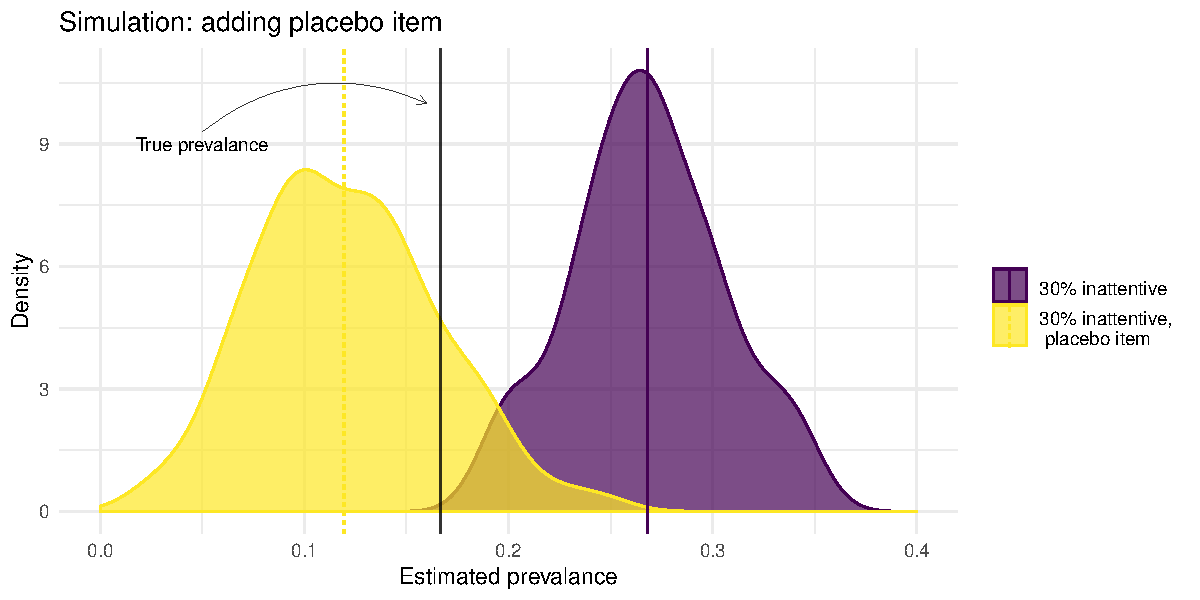
\includegraphics[width=6.25in,height=\textheight]{output/estimates_placebo_color.pdf}
\caption{Simulation of \(\hat{\tau}\) by adding a placebo item. 10000
simulated data sets. \label{placebo_simulation}}
\end{figure}

\hypertarget{list-effect-bias}{%
\section{List effect bias}\label{list-effect-bias}}

In list experiment B and E respondents are randomly assigned to one of
three groups: a ``normal'' control group, a control group receiving the
placebo item, and the treatment group receiving the ``sensitive'' item.
We define list effect bias as the difference between any list effect in
a list with \(J\) items and a list with \(J+1\) items. We denote this
bias \(\Delta L\). To test for the presence of \(\Delta L\) we first
exclude inattentive respondents and then compare the normal control list
to the control list with a placebo item. In the absence of list effect
bias this difference should be close to 0.

List effect bias implies that respondents given the longer list adjust
their response in a way that that respondents assigned to the shorter
list do not. To simulate this process we assume that respondents
assigned to the normal control list respond according to their true
preference for the control items denoted by \(Z_{ij}\). Like in previous
simulations we assume that each individual item is a draw from a
Bernoulli distribution where the parameter \(p_{j}\) was set to 0.5,
0.5, 0.15, and 0.85 for the different items respectively. We assume that
``respondents'' in the placebo control group answer affirmatively to
each item with the same probability, and never answer affirmatively to
the placebo item. However, conditional on giving a ``low'' response
these respondents adjust their answer upwards by one item (simulating
positive list effect bias) with probability \(p_{l}\). A response is
``low'' when the total number of affirmative answers is below som
threshold \(j_{low}\). For respondents in the normal control group the
response is generated by: \(Y^*_{i} = \sum_{j=1}^{J} Z_{ij}\). For
respondents in the treatment group the response is generated by
\(Y^*_{i} = \sum_{j=1}^{J} Z_{ij} + \mathbbm{1}_{ \{ \sum_{j=1}^{J} Z_{ij}<j_{low} \} } X_{l}\).
Where \(\mathbbm{1}\) is the indicator function and
\(X_{l} \sim Bernoulli(p_{l})\). Under this setup \(\Delta L\) will be
equal to \(p(\sum_{j=1}^{J} Z_{ij}<j_{low}) \times X_{l}\).

To roughly estimate the power of our test to detect list effect bias
(see above) we run the following simulation. We assume 4000 respondents.
We assume that \(s=0.25\) and therefore exclude 1000 ``inattentive''
respondents from the sample, leaving 3000 respondents (hence around 1000
respondents in each group). We set \(j_{low}\) to 3 and \(p_{l}\) to
\(0.1\), indicating that respondents given the placebo list who would
answer below 3 have a probability of 0.1 to adjust their answer upwards
by one item. Under this setup the test comparing the difference between
the two control lists (using the DiM estimator) has a 75\% chance to
reject the null hypothesis. Using the same simulation setup and a
sensitive item with a prevalence of \(\frac{1}{6}\) for the treatment
group, we estimate that the chance that the \(pRMSE(\hat{\tau})\) will
be lower when estimating \(\tau\) using the placebo control group as
compared to the normal control group is 93\%.

\newpage

\hypertarget{question-wording}{%
\section{Question wording}\label{question-wording}}

\begin{longtabu} to \linewidth {>{\bfseries\raggedright\arraybackslash}p{10em}|>{\raggedright\arraybackslash}p{35em}}
\caption{\label{tab:unnamed-chunk-1}Does this work? \label{full-survey} }\\
\toprule
Tag & Wording\\
\midrule
intro & 感谢您的参与! 
此项社会科学调查在哥德堡大学研究员的监督下开展。您的参与将为学术研究做出非常有价值的贡献。  您的参与将对学术研究提供很有价值的贡献。所以您仔细阅读所有问题并且诚实回答这些问题是非常重要的。如果您不想回应一个问题,那么请选择“不想回答”。完成这份问卷会占用您大约 10 分钟的时间。参与这个调查是完全自愿的,而且未经授权的人员无法获得您的回答。如果任何时候您希望放弃这次调查则您可以转换到其它网页或者关闭浏览器窗口。 如果您希望参与那么请点击下面的“下一页”。如果您不希望参与那么您可以转换到其它网页或者关闭浏览器窗口。\\
age & 您多大年纪?\\
gender & 性别:\\
hukou & 您现在的户口类型是什么?\\
IMC\_1 & 我们想要了解一下您的喜好。现代决策论认为人们的种种决定不是凭空做出的。为了显示您已经仔细阅读了这部分题目,请忽略您的个人喜好,选择下面的红色和绿色。您不用思考下面的题目,请直接选择这两个颜色。您最喜欢的颜色是什么?\\
\addlinespace
income & 年薪收入(人民币)?\\
education & 您的最高学历是什么?\\
work & 您是在政府或国有企事业单位工作,还是在私营企业单位工作?\\
party & 政治面貌?\\
info & 您将在下看到一系列表述。请说明您是否赞同或反对各项表述。\\
\addlinespace
imc\_2\_1 & 请点击“说不上同意或反对”选项\\
imc\_2\_2 & 中国国旗的主要颜色是绿色\\
imc\_2\_3 & 杀人犯应被判死刑\\
imc\_2\_4 & 同性恋应该享受合法婚姻的权力\\
imc\_2\_5 & 为了家庭,个人应该把他或她自身的利益放在第二位\\
\addlinespace
imc\_2\_6 & 作为一名学生,一个人不应该质疑老师的权威\\
imc\_2\_7 & 即使父母的要求不合理,子女也应该去做他们要求的事情\\
audit & 为了确保受访者已阅读说明、并认真地回答问题,接下来会有一些非常简单的问题,以便测试您是否已经阅读了说明。为了数据的准确性,我们只会接受明确表明了自己已经阅读并理解本次调查的受访者。如果您答错了,我们可能无法使用您的数据。您明白了吗?\\
list\_intro & 现在,我们想了解在下列表述中,您赞同或者认可其中的多少项?您无需指出具体哪一项,只需要告诉我们您总共赞同多少项。\\
a\_1 & 在我们国家,空气污染是一个重要的问题。\\
\addlinespace
a\_2 & 我小时候经常和祖父母/外祖父母在一起。\\
a\_3 & 总体而言, 我国的生活质量比30年前低。\\
a\_4 & 经济发展比保护环境更重要。\\
a\_control & 请指出您赞同以上多少项表述:\\
list\_intro & 现在,我们想了解在下列表述中,您赞同或者认可其中的多少项?您无需指出具体哪一项,只需要告诉我们您总共赞同多少项。\\
\addlinespace
a\_1 & 在我们国家,空气污染是一个重要的问题。\\
a\_2 & 我小时候经常和祖父母/外祖父母在一起。\\
a\_3 & 总体而言, 我国的生活质量比30年前低。\\
a\_4 & 经济发展比保护环境更重要。\\
season\_1 & 我出生在冬季(12月/1月/2月)\\
\addlinespace
season\_2 & 我出生在春季(3月/4月/5月)\\
season\_3 & 我出生在夏季(6月/7月/8月)\\
season\_4 & 我出生在秋季(9月/10月/11月)\\
a\_treatment & 请指出您赞同以上多少项表述:\\
fmc\_a & 您刚刚回答了一个问题,从一系列表述中选择了自己赞同的项目。以下有四项表述。其中只有一项出现在了之前的列表中。是哪一项?请选择该项,无论它是否属于您赞同的其中一项。\\
\addlinespace
list\_intro & 现在,我们想了解在下列表述中,您赞同或者认可其中的多少项?您无需指出具体哪一项,只需要告诉我们您总共赞同多少项。\\
b\_1 & 政府是人民的公仆,应该按人民的意愿做事。\\
b\_2 & 政府就像是家长,应该告诉人民应该做什么。\\
b\_3 & 我现在生活的城市就是我的出生地。\\
b\_4 & 通常来说,大部分人都不能被信任。\\
\addlinespace
zodiac\_1 & 我出生在鼠年或牛年。\\
zodiac\_2 & 我出生在虎年或兔年。\\
zodiac\_3 & 我出生在龙年或蛇年。\\
zodiac\_4 & 我出生在马年或羊年。\\
zodiac\_5 & 我出生在猴年或鸡年。\\
\addlinespace
zodiac\_6 & 我出生在狗年或猪年。\\
b\_treatment & 请指出您赞同以上多少项表述:\\
intro\_list & 现在,我们想了解在下列表述中,您赞同或者认可其中的多少项?您无需指出具体哪一项,只需要告诉我们您总共赞同多少项。\\
b\_1 & 政府是人民的公仆,应该按人民的意愿做事。\\
b\_2 & 政府就像是家长,应该告诉人民应该做什么。\\
\addlinespace
b\_3 & 我现在生活的城市就是我的出生地。\\
b\_4 & 通常来说,大部分人都不能被信任。\\
placebo\_1 & 我出生于21世纪00年代。\\
placebo\_2 & 我出生于20世纪70年代。\\
b\_placebo & 请指出您赞同以上多少项表述:\\
\addlinespace
intro\_list & 现在,我们想了解在下列表述中,您赞同或者认可其中的多少项?您无需指出具体哪一项,只需要告诉我们您总共赞同多少项。\\
b\_1 & 政府是人民的公仆,应该按人民的意愿做事。\\
b\_2 & 政府就像是家长,应该告诉人民应该做什么。\\
b\_3 & 我现在生活的城市就是我的出生地。\\
b\_4 & 通常来说,大部分人都不能被信任。\\
\addlinespace
b\_control & 请指出您赞同以上多少项表述:\\
fmc\_b & 您刚刚回答了一个问题,从一系列表述中选择了自己赞同的项目。以下有四项表述。其中只有一项出现在了之前的列表中。是哪一项?请选择该项,无论它是否属于您赞同的其中一项。\\
intro\_list & 现在,我们想了解在下列表述中,您赞同或者认可其中的多少项?您无需指出具体哪一项,只需要告诉我们您总共赞同多少项。\\
c\_1 & 女性像男性一样能成为好的政治领导\\
c\_2 & 遵循宗教标准和仪式很重要。\\
\addlinespace
c\_3 & 当工作稀缺的时候,男性应该比女性更有权利获得一份工作。\\
c\_4 & 我国应该增加商业的私有制。\\
c\_sensitive & 我信任常驻北京的国家政府。\\
c\_treatment & 请指出您赞同以上多少项表述:\\
list\_intro & 现在,我们想了解在下列表述中,您赞同或者认可其中的多少项?您无需指出具体哪一项,只需要告诉我们您总共赞同多少项。\\
\addlinespace
c\_1 & 女性像男性一样能成为好的政治领导。\\
c\_2 & 遵循宗教标准和仪式很重要。\\
c\_3 & 当工作稀缺的时候,男性应该比女性更有权利获得一份工作。\\
c\_4 & 我国应该增加商业的私有制。\\
c\_control & 请指出您赞同以上多少项表述:\\
\addlinespace
list\_intro & 现在,我们想了解在下列表述中,您赞同或者认可其中的多少项?您无需指出具体哪一项,只需要告诉我们您总共赞同多少项。\\
d\_1 & 媒体发布新闻和观点时,应有权不受政府控制。\\
d\_2 & 我家之前几年的经济状况比现在要好。\\
d\_3 & 总体来说,我们国家正在走向正确的发展方向。\\
d\_4 & 如果人们有太多各种各样的想法,社会会变得混乱。\\
\addlinespace
d\_sensitive & 我信任我的本地政府。\\
d\_treatment & 请指出您赞同以上多少项表述:\\
list\_intro & 现在,我们想了解在下列表述中,您赞同或者认可其中的多少项?您无需指出具体哪一项,只需要告诉我们您总共赞同多少项。\\
d\_1 & 媒体发布新闻和观点时,应有权不受政府控制。\\
d\_2 & 我家之前几年的经济状况比现在要好。\\
\addlinespace
d\_3 & 总体来说,我们国家正在走向正确的发展方向。\\
d\_4 & 如果人们有太多各种各样的想法,社会会变得混乱。\\
d\_control & 请指出您赞同以上多少项表述:\\
intro\_list & 现在,我们想了解在下列表述中,您赞同或者认可其中的多少项?您无需指出具体哪一项,只需要告诉我们您总共赞同多少项。\\
e\_1 & 我对政治非常感兴趣。\\
\addlinespace
e\_2 & 富人和穷人没有受到政府的平等对待。\\
e\_3 & 我去过北京。\\
e\_4 & 政府为所有人提供优质的公共服务。\\
e\_sensitive & 去年我被要求贿赂某位政府官员。\\
e\_treatment & 请指出您赞同以上多少项表述:\\
\addlinespace
intro\_list & 现在,我们想了解在下列表述中,您赞同或者认可其中的多少项?您无需指出具体哪一项,只需要告诉我们您总共赞同多少项。\\
e\_1 & 我对政治非常感兴趣。\\
e\_2 & 富人和穷人没有受到政府的平等对待。\\
e\_3 & 我去过北京。\\
e\_4 & 政府为所有人提供优质的公共服务。\\
\addlinespace
e\_control & 请指出您赞同以上多少项表述:\\
intro\_list & 现在,我们想了解在下列表述中,您赞同或者认可其中的多少项?您无需指出具体哪一项,只需要告诉我们您总共赞同多少项。\\
e\_1 & 我对政治非常感兴趣。\\
e\_2 & 富人和穷人没有受到政府的平等对待。\\
e\_3 & 我去过北京。\\
\addlinespace
e\_4 & 政府为所有人提供优质的公共服务。\\
placebo\_3 & 我出生于20世纪60年代。\\
placebo\_4 & 我出生于20世纪90年代。\\
e\_placebo & 请指出您赞同以上多少项表述:\\
fmc\_e & 您刚刚回答了一个问题,从一系列表述中选择了自己赞同的项目。以下有四项表述。其中只有一项出现在了之前的列表中。是哪一项?请选择该项,无论它是否属于您赞同的其中一项。\\
\addlinespace
placebo\_1\_direct & 您是否同意下列说法? ""我出生于21世纪00年代""。\\
placebo\_2\_direct & 您是否同意下列说法? ""我出生于20世纪70年代""。\\
non\_sens\_direct & 您是否同意下列说法? ""总体来说,大多数人是值得信任的""。\\
c\_direct & 您是否同意下列说法? ""我信任常驻北京的国家政府""。\\
d\_direct & 您是否同意下列说法? ""我信任我的本地政府""。\\
\addlinespace
e\_direct & 您是否同意下列说法? ""去年我被要求贿赂某位政府官员""。\\
sponsor & 最后一个问题. 您认为是谁委托进行了这次调查研究?\\
end & 感谢您抽时间参与本次调查。您的回答已被记录。\\
\bottomrule
\end{longtabu}


\end{document}
